\section{Beyond Benchmarks}
\label{sec:beyondbenchmarks}

\ours demonstrates its iterative feedback and refinement capabilities in the context of website layout generation. \chatgpt initially produces a rudimentary layout for a given topic, and then uses the \fbmod to suggest specific, actionable improvements, as demonstrated in \Cref{fig:website:ice_cream_init,fig:website:photo_init}. These suggestions range from design changes such as color and font adjustments, to content enhancements and layout modifications. \Cref{fig:website:ice_cream_refined,fig:website:photo_refined} showcase the final layouts, post-feedback implementation, highlighting the potential and versatility of \ours across different scenarios.

\begin{figure}[!ht]
    \centering
    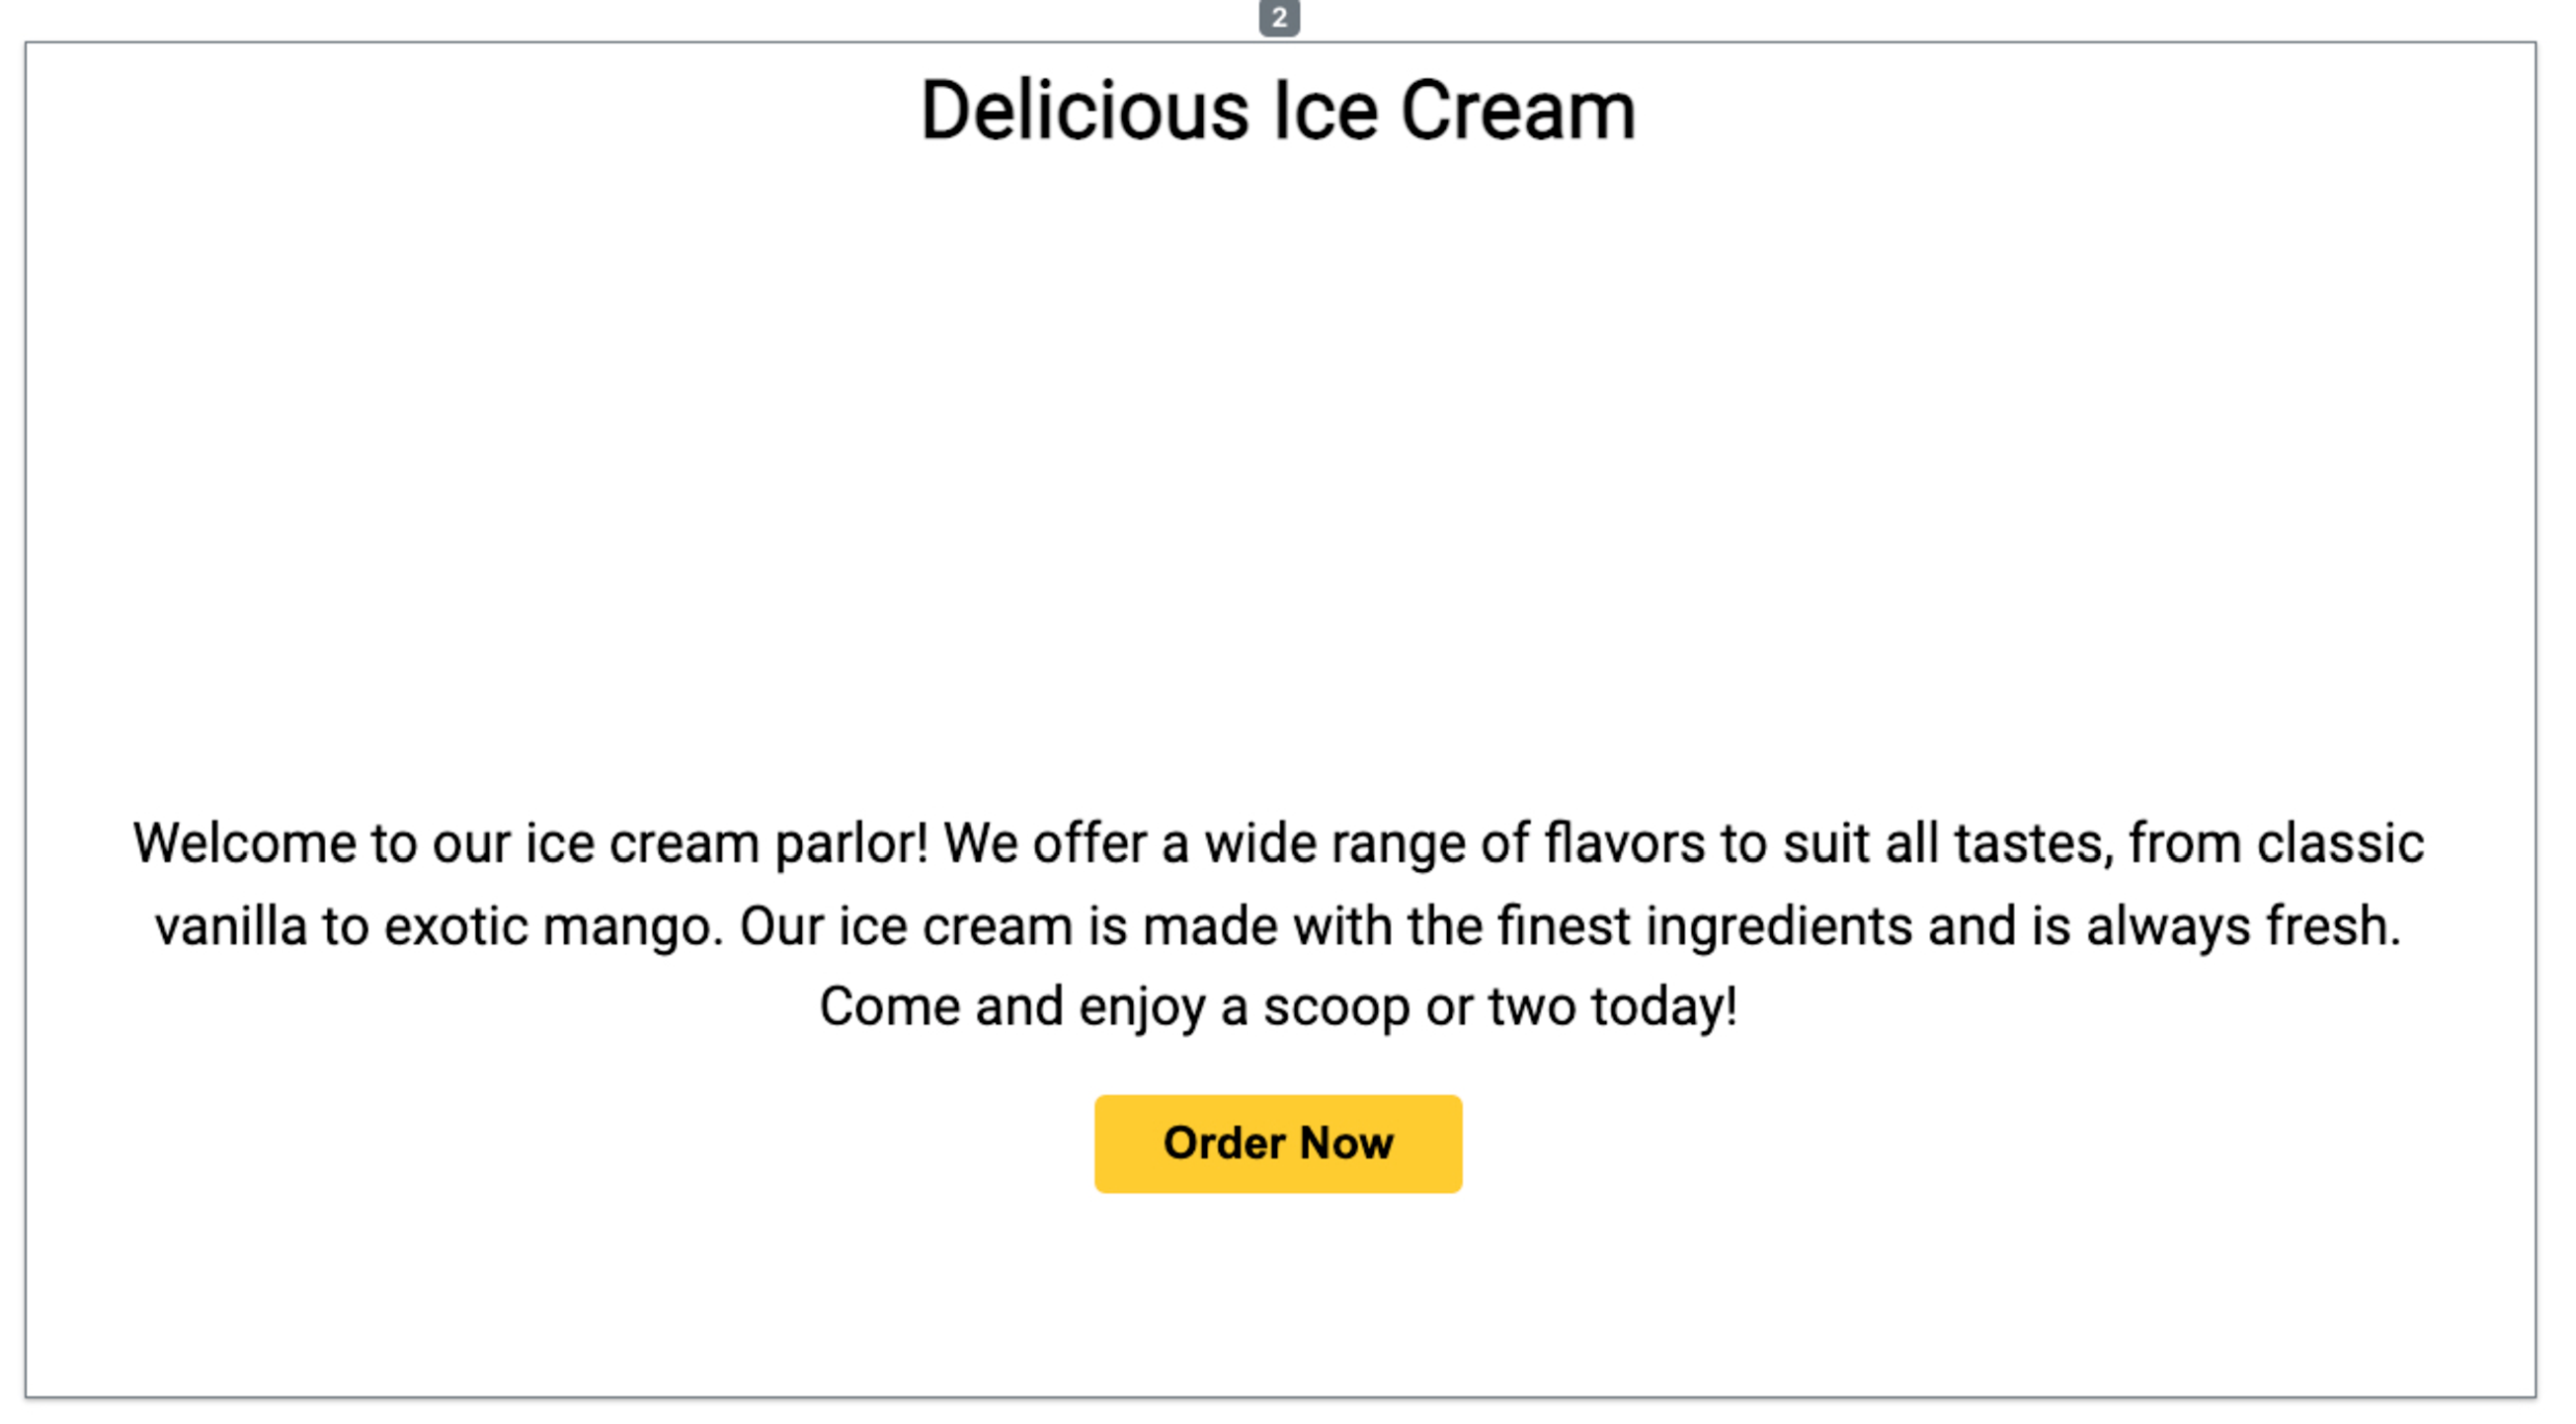
\includegraphics[scale=0.3]{figures/website-generation/ice_cream_init.pdf}
    \caption{Initial web layout generated by our model for a fictional ice cream parlor.}

    \label{fig:website:ice_cream_init}
\end{figure}


\paragraph{Ice Cream Generation}

The feedback generated by \fbmod for ice cream generation:
\squishlist
\item Change the background color of the container to a light blue color (\#6f2ff).
\item Change the font size of the heading to 48px.
\item Add a small icon before the "Welcome to our ice cream parlor!" text using the URL https://cdn-icons-png.flaticon.com/512/3622/3622340.png.
\item Add an additional paragraph after the existing text with the following text: "We also offer a variety of toppings and cones to complement your ice cream. Visit us today to try our latest flavors and indulge in a sweet treat!"
\item Increase the font size of the button text to 24px.
\item Update the button color to \#9933.
\squishend


\begin{figure}[!ht]
    \centering
    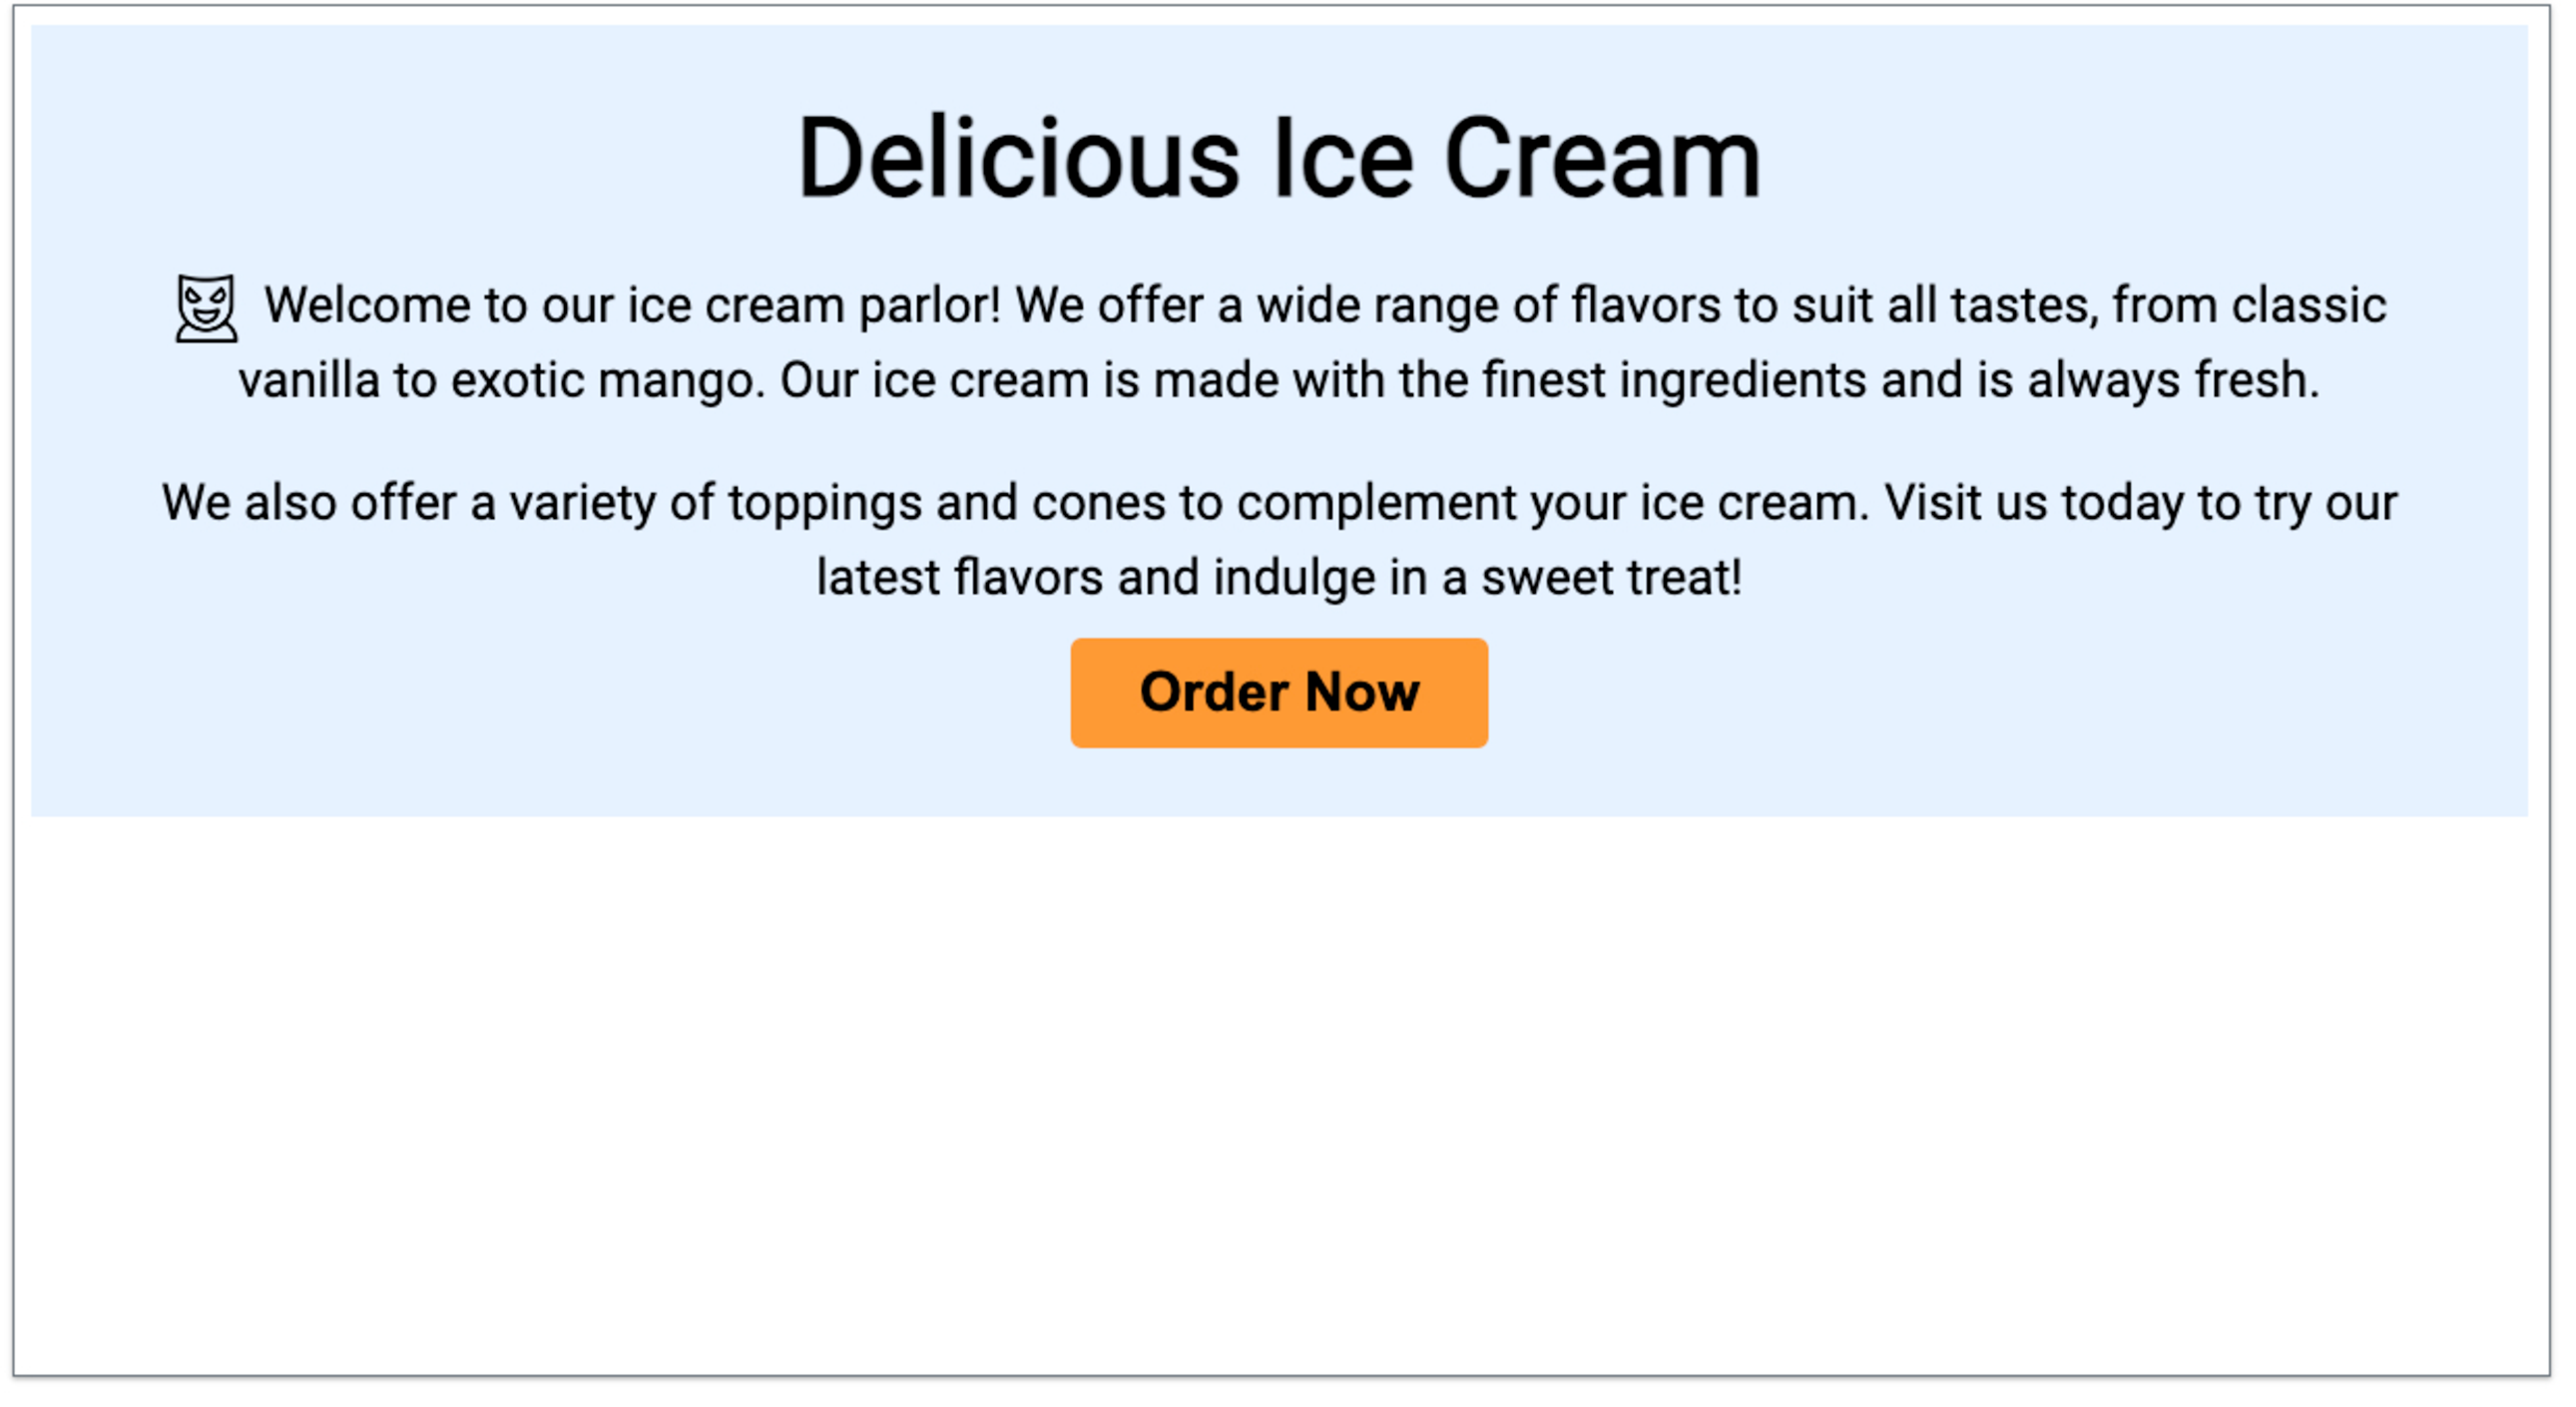
\includegraphics[scale=0.3]{figures/website-generation/ice_cream_refined.pdf}
    \caption{Refined web layout after applying model feedback. The feedback included changing the background color to light blue (\#6f2ff), increasing the heading font size to 48px, adding an icon before the welcome text, enhancing the content with an additional paragraph, increasing the button text size to 24px, and updating the button color to \#9933.}
    \label{fig:website:ice_cream_refined}
\end{figure}




\begin{figure}[!ht]
    \centering
    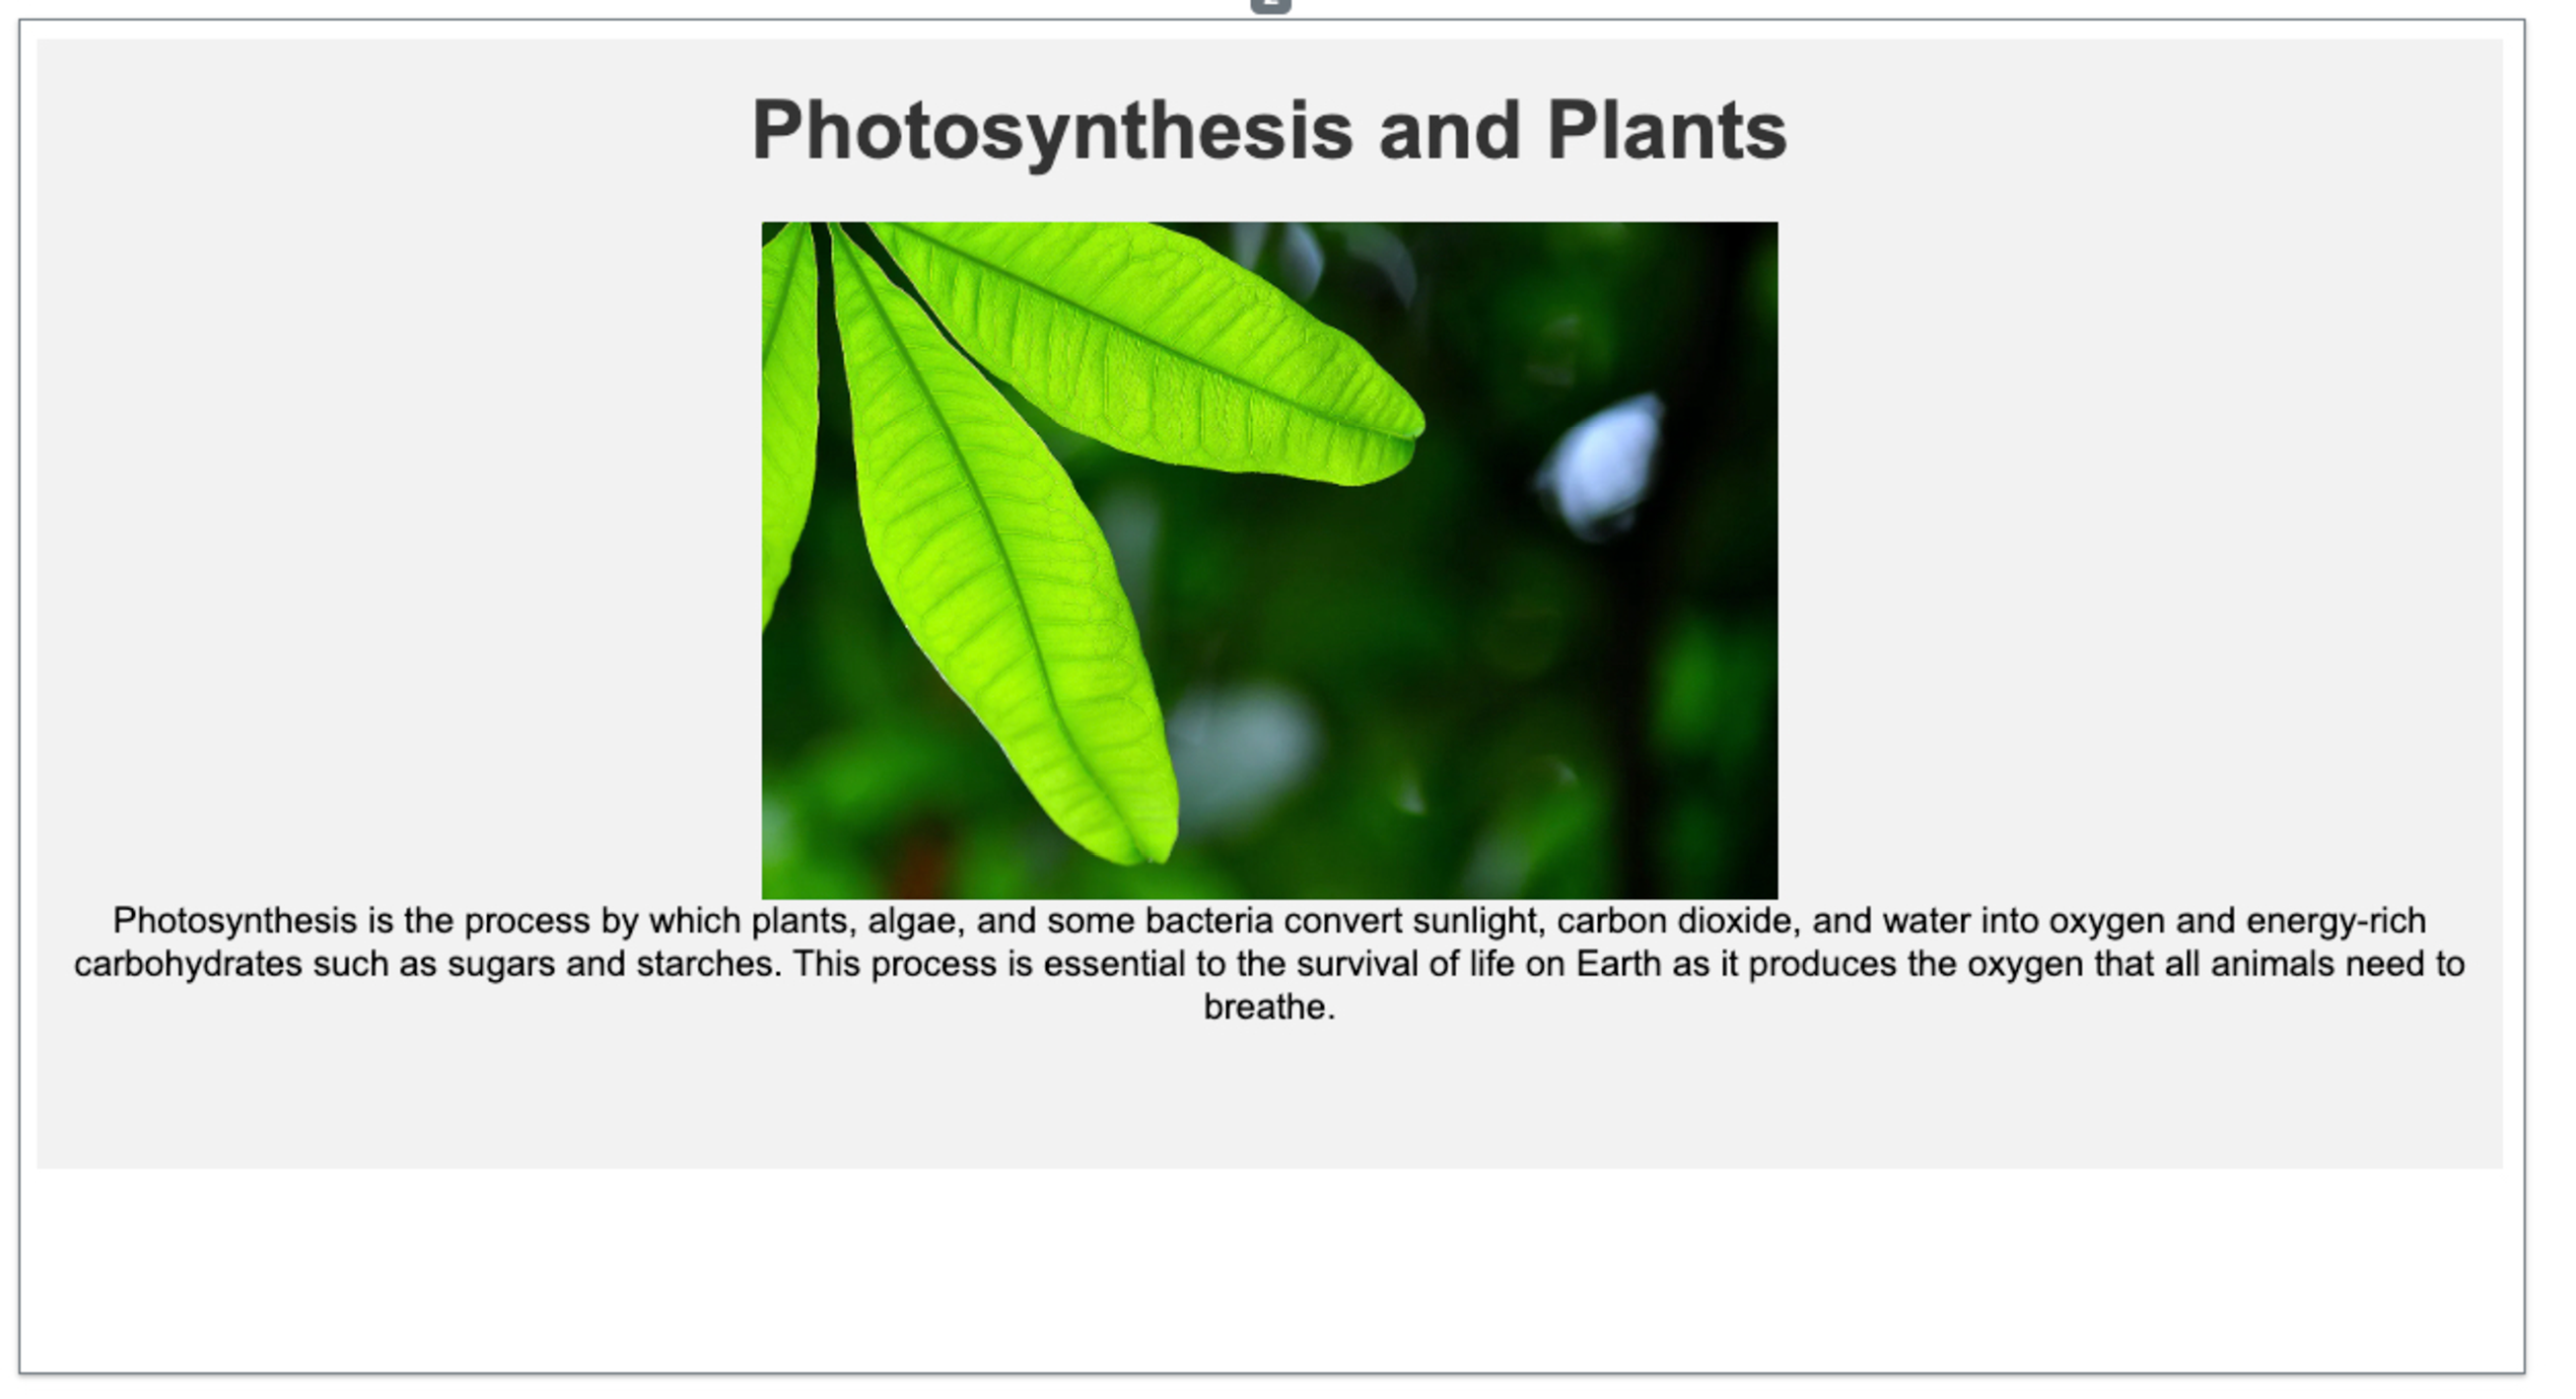
\includegraphics[scale=0.3]{figures/website-generation/photo_init.pdf}
    \caption{Initial web layout generated by our model for a page on photosynthesis.}
    \label{fig:website:photo_init}
\end{figure}

\paragraph{Photosynthesis}

The feedback generated by \fbmod for photosynthesis:
\squishlist
\item Increase the font size of the text to 18px for better readability.
\item Add more information about the benefits of photosynthesis.
\item Remove the unnecessary margin-top from the header.
\item Add a ruler or divider below the header to separate it from the image.
\squishend


\begin{figure}[!ht]
    \centering
    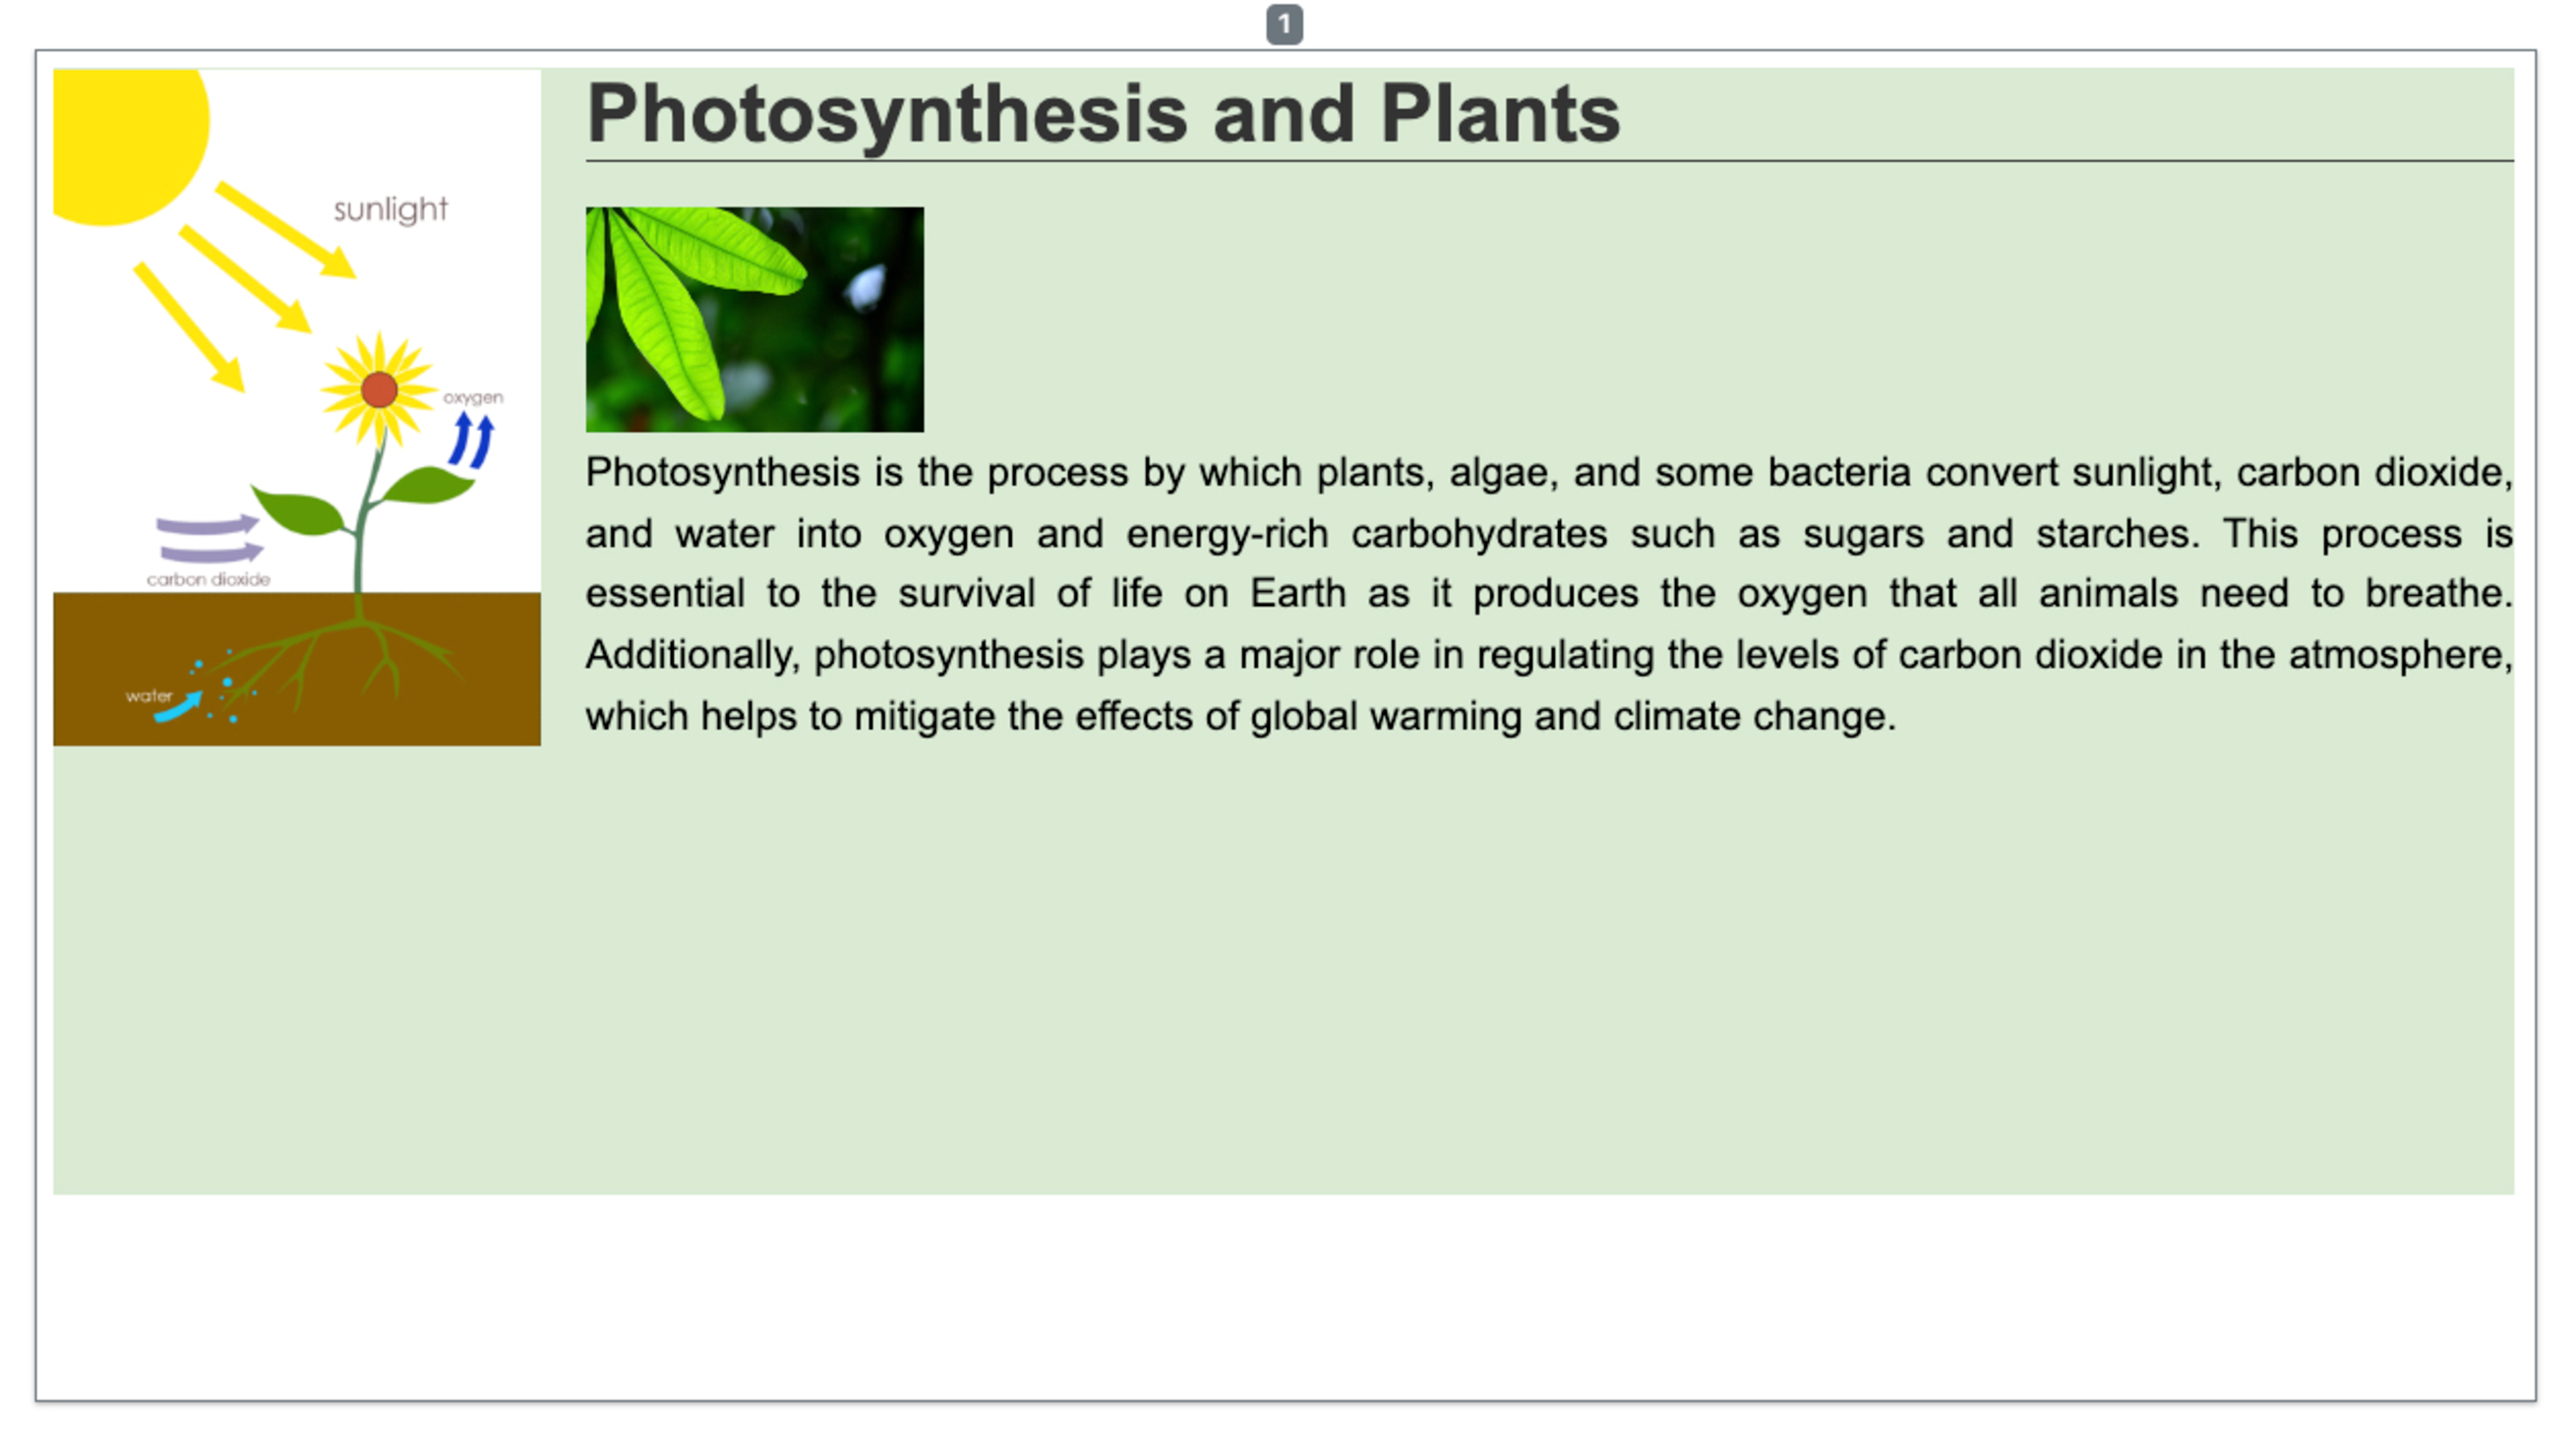
\includegraphics[scale=0.3]{figures/website-generation/photo_refined.pdf}
    \caption{Refined web layout after applying model feedback. The feedback included increasing the text font size to 18px for better readability, adding more information about the benefits of photosynthesis, removing the unnecessary margin-top from the header, and adding a ruler or divider below the header to separate it from the image.}
    \label{fig:website:photo_refined}
\end{figure}